\documentclass[submit, 12pt]{aiaa-pretty-modified}

\usepackage{graphicx}
\usepackage{array}
\usepackage{amsmath}
\usepackage{amssymb}
\usepackage{multirow}
\usepackage{rotating}
\usepackage[header,page]{appendix}
\usepackage{placeins}
\usepackage{pdfpages}
\usepackage[notbib]{tocbibind}
\usepackage{setspace}
\usepackage[tocindentauto]{tocstyle}

\usetocstyle{standard}

\title{\textbf{Planning Algorithms for Indoor Robotic Odor
    Localization}\\
{16.622 Final Report}}

\date{\today}

\author{Authors: \\Troy Astorino \\ Mark Van de Loo \\
  \\ 
  Advisors:\\ Professor Youssef Marzouk \\ Professor Nicholas
    Roy \\ Josh Joseph \\ Javier Velez \\ Xun Huan \\ Sachi Hemachandra}

\newcommand{\tablewidth}[0]{1in}
\newcommand{\tablewidthtwo}[0]{3in}
\newcount\colveccount
\newcommand*\colvec[1]{
  \global\colveccount#1
  \begin{pmatrix}
    \colvecnext
  }
  \def\colvecnext#1{
    #1
    \global\advance\colveccount-1
    \ifnum\colveccount>0
    \\
    \expandafter\colvecnext
    \else
  \end{pmatrix}
  \fi
}

% \makeatletter
%   \renewcommand\l@subsection{\@dottedtocline{2}{1.5em}{3em}}
% \makeatother
  
\begin{document}
\maketitle

\newpage

\tableofcontents

\newpage

\listoffigures

\newpage

\listoftables

\newpage
\onehalfspace

\section{Introduction}

Odor localization is defined as ``the act of finding the location of a
volatile chemical source in the environment.''\cite{kowadlo} Odor
localization is an essential process for many biological systems, from
moths following pheromone trails to find mates, to bacteria finding a
food source. The field of robotic odor localization, which has drawn
much inspiration from biological processes, promises many benefits to
humanity today. Robots could use odor localization to accomplish tasks
in environments that would prove dangerous for humans: finding the
source of toxic chemical leaks for instance, or finding people
trapped in a collapsed building or mine.

There has been little robotic odor localization research done in indoor
environments. This is due to the difficulty of modeling turbulence in a typical
room. Accurate prediction of airflow requires precise knowledge of the geometry
and ventilation of the room, and even if these are known, prediction is too
computationally expensive to perform in real-time on a robot. Instead of trying
to precisely predict how airflows affect indoor vapor dispersion, this
experiment will attempt to use localization algorithms robust enough to overcome
transient turbulence introduced by indoor air currents. Our experiment will
address the problem of odor localization in irregularly shaped rooms through the
use of gradient descent approaches to autonomous path planning.

\section{Hypothesis, Objective, Success Criteria}
\label{sec:hos}
\subsection*{Hypothesis} 
The mean localization rate of a 45-minute two-dimensional search by an
autonomous ground robot equipped with a chemical vapor sensor will be 20 percent
greater using a stochastic planner than using a simple gradient descent planner.
\footnote{ The greedy gradient descent algorithm always moves the robot in the
  direction of the best source estimate. A stochastic algorithm moves to a
  location randomly sampled from source estimate probability distribution,
  allowing the planning algorithm to gain a more complete representation of the
  search space, at the potential cost of taking some unnecessary measurements.}

\subsection*{Objective}
Equip a ground robot furnished by the CSAIL Robust Robotics Group with an Alpha MOS NEEM chemical sensor, implement the planners on the robot's software platform, and assess the mean localization rate of a cup of ethanol in a closed room.

\subsection*{Success Criteria} 
Determine the difference in mean localization rate to a sufficient precision such that the hypothesis can be assessed.

\section{Literature Review}
Approaches to robotic odor localization may be analyzed as a combination of
three components: a model, an estimator, and a planner. The model is a
mathematical function that describes the spatiotemporal variation of the
chemical concentration. The estimator represents the process by which
measurements of the chemical concentration are combined with model in real time
to obtain an estimate of the location of the chemical source. The planner is an
algorithm that decides the location of the next measurement given the current
estimate and confidence interval of the source location.

Review of previous work in the field of robot odor localization helped to select
this experiment's test environment of windless indoor rooms with uncommon
geometries. In addition, it provided the basis for the selection of a Bayesian inference
estimator and a Gaussian model to be selected as parameters of the experiment, and
motivated the selection of a simple gradient descent planner and a stochastic
gradient descent planner as interchangeable parts of the localization algorithm
to be compared for speed.

\subsection{Experiment Motivation}
Robotic odor localization experiments have been conducted using chemical
dispersion in water, air, and soil.\cite{kowadlo} In water and soil, diffusion is the
dominating method by which a chemical emanates from a source and disperses
through space. In air, where the Reynolds number is higher than in water or
soil, the behavior of the chemical concentration is affected by the presence of
turbulent fluid currents in addition to chemical diffusion.\cite{kowadlo} These turbulent
currents have led most robotic odor localization researchers to introduce an
artificial wind source when working in air. This negates the effect of the
turbulence, producing a concentration plume that behaves as a 2-dimensional
Gaussian function in planes normal to the wind direction, and downwind of the
source. \cite{ferri} While smoothing the concentration field in this manner makes the task of locating the
chemical source more straightforward, this environment is not representative of
a realistic indoor scenario. A few experiments, such as that done by Ferri, et
al., have been conducted in an indoor environment without an artificial wind
source. \cite{ferri} In general, however, it seems that turbulent indoor environments
have been less explored than their artificial wind source counterparts. For this
reason, it was decided that this experiment will be conducted in an ambient,
windless indoor environment. In addition, the experiment will attempt robot odor
localization in test rooms with floor plans that are not rectangular and have
non-intuitive geometries, which to the knowledge of the authors has not been done
previously.

\subsection{Selection of Model and Estimator}
Due to the varying effects of turbulence and diffusion discussed in section 3.1,
accurate modeling of the concentration field is dependent upon the medium and
environment in which the experiment is conducted. However, many robotic odor
localization researchers chose not to use a high-fidelity model of the
concentration field, deeming this level of complexity unnecessary. \cite{kowadlo} Most
commonly used was a dispersion model based on a Gaussian function. Time
invariant Gaussian models were used successfully in experiments in water and
soil, as well as in air with an artificial wind source. \cite{kowadlo} In turbulent air,
Ferri, et al. successfully used a time invariant monotonic function with a
single peak at the source location as a concentration model. \cite{ferri} The two
algorithms tested both successfully localized a dish of ethanol in a mean time
of less than 10 minutes, beginning an average distance of 1.8m from the source.
The model used in these localization algorithms is not explicitly described in
\cite{ferri}, but the assumption that the model is time invariant and monotonic with a
single peak is a defining component of the successful localization algorithms
presented in this paper. Based on the success of Ferri, et al., it was decided
that this experiment would use a Gaussian concentration field model, treating
the effects of turbulent fluid currents in the air as noise. A Bayesian filter
was selected as an estimator to account for this noise in determining a
probability distribution of the source location after each measurement. The
Bayesian filter is a common technique used in conjunction with Gaussian models
in robotic localization and is described in \cite{bergman}.

\subsection{Selection of Planners}
Planners that were shown to be effective in turbulent air environments were
mainly derived from observations of the behavior of biological organisms.
\cite{ferri} For example, Ferri et al. attempted to mimic the circling behavior
of the Luna Moth in its search for a mate in one planner, and the weighted
random walk exhibited by the chemotaxis of the E. coli bacterium in another.
\cite{ferri} No documentation of simple gradient descent using a single sensor
or other simple statistically motivated planners as applied to robot odor
localization was found. Using simple gradient descent is attractive because of
its simplicity, but due to the turbulent nature of ambient indoor air, a simple
gradient descent planner may be prone to confusion by temporary local maxima of
the chemical concentration. An alternative planner that may perform better in
the turbulent environment without requiring a complicated model is based on
stochastic gradient descent, which adds randomness to the gradient vector when
prescribing the direction of motion. \cite{bottou} This randomness may
help avoid
the issues caused by temporary local maxima.

\section{Description of Experiment}
\subsection{Experimental Overview}
A simple gradient descent (greedy) planning aglorithm and a
stochastic planning algorithm were tested using the
same model and estimation method. A sensor capable of identifying the
concentration of ethanol in the surrounding air was mounted on a ground
robot. A dish of ethanol was placed in a test room, and the mean rate at which the robot localized the ethanol source
using the greedy planner was compared to the mean rate using the
stochastic planner.

\subsection{Test Apparatus}
\label{sec:design}
\subsubsection{Hardware and Robot Platform}

The Alpha MOS NEEM chemical sensor shown in figure \ref{fig:sensor} was
attached to the Envoy robotic platform of the Robust Robotics Group, illustrated in figure \ref{fig:wheelchair}.  The sensor was mounted
30 cm above the ground.


\begin{figure}
\begin{center}
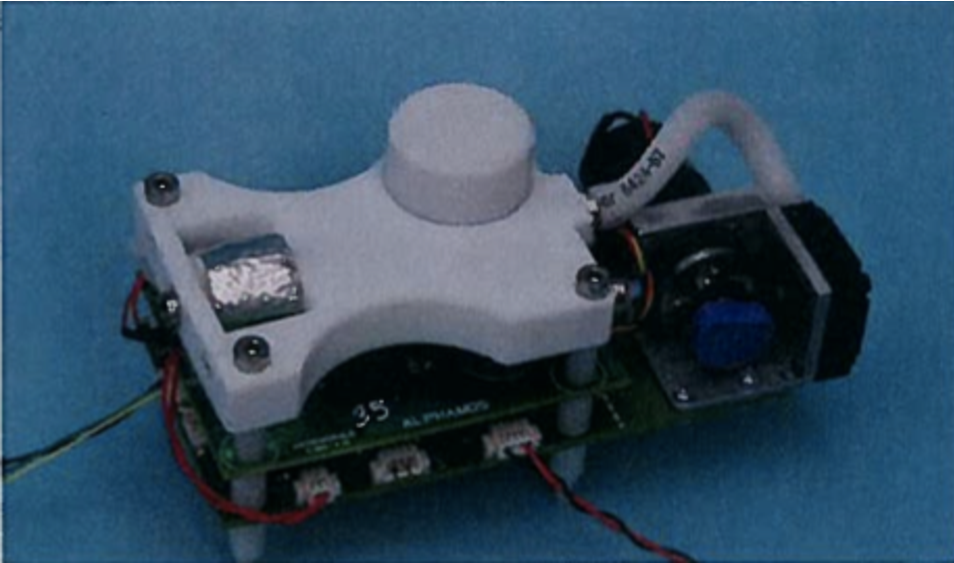
\includegraphics[width=3in]{img/sensor.pdf}
\caption{Alpha MOS NEEM chemical sensor.}
\label{fig:sensor}
\end{center}
\end{figure}

A laptop computer
mounted on the robot performed all real-time computation and data
collection.  The robot used two LIDARs and a pre-loaded map of the
test room to determine its position.  The position was made available
as telemetry to the estimator via the LCM messaging protocol at a rate
of 40 hz as
illustrated in figure \ref{fig:acquisition}.

\begin{figure}
\begin{center}
\includegraphics[width=5in]{img/wheelchair.pdf}
\caption{Envoy robotic wheelchair platform with Alpha MOS Neem Sensor.}
\label{fig:wheelchair}
\end{center}
\end{figure}

\FloatBarrier

\label{sec:mount}

\subsubsection{System Control Flow}

After reaching each measurement location commanded by the planner,
the robot entered a waiting period of 30 seconds to allow transient
concentration behaviors and sensor dynamics to attenuate before
beginning to take readings.  This period was followed by another 30
second period during which readings of the chemical vapor
concentration were recorded at a rate of 1 hz.  These readings were
averaged, and the natural logarithm of the average was passed to the
estimator.  The estimator then used this value and the current
position of the robot to update its posterior belief.  This belief was
then passed to the planner, which issued the next commanded
measurement location to the robot.  The robot moved to that measurement
location, and began the process again.  Data flow between the components of the system is illustrated in
Figure \ref{fig:acquisition}.

\begin{figure}
\begin{center}
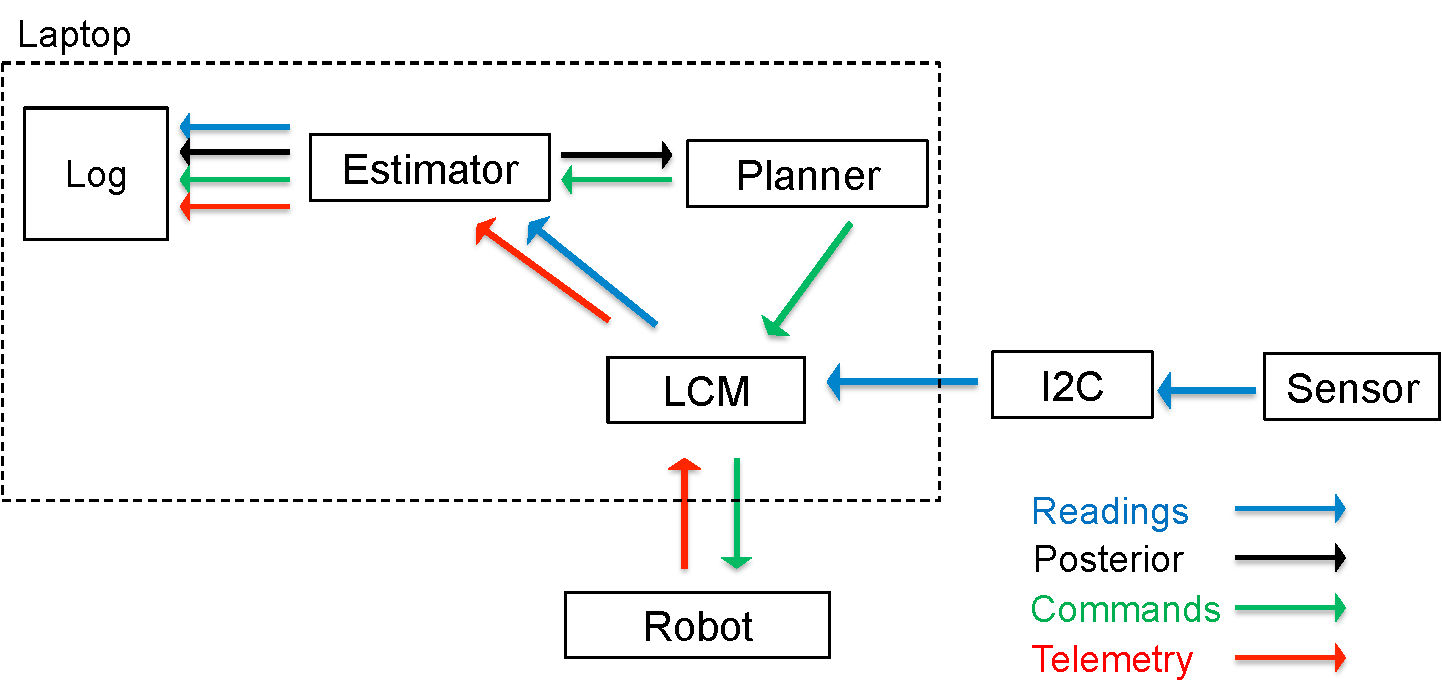
\includegraphics[width=6in]{img/acquisition.pdf}
\caption[Data acquisition flowchart]{The components of the system, and the paths along which data is
  communicated. Messages are passed among different components of the robot's
  software using the LCM protocol.  Sensor readings include a raw
  chemical concentration value.  The
  posterior distribution is the robot's current best estimate of the chemical
  source's location. Commands are sent in the form of a target position and
  orientation of the robot. Telemetry includes the robot's position, velocity,
  and attitude.}
\label{fig:acquisition}
\end{center}
\end{figure}

\subsubsection{Estimator}

The estimate of the source location was calculated using a particle
filter\cite{maskell2001tutorial}. The particles were distributed with uniform
spacing over the area of the test room, and each particle held the posterior
estimate's belief that the source is at it's location. The particle density is listed in Table
\ref{tab:estimator-parameters}. After each concentration measurement was
received, a Bayesian update was performed on each particle: 
\[P_n(x_i = x_s) \propto P(c_n | x_i = x_s) P_{n-1}(x_s = x_i)\]
In the above expression, $P_n(x_i = x_s)$ is the posterior belief that the source is located at the
$i^{th}$ particle location after the $n^{th}$ update. $c_n$ is the $n^{th}$ concentration
measurement taken. $P(c_n | x_i = x_s)$ is the likelihood function, the probability that $c_n$ is
measured given that the source is at the $i^{th}$ particle location according to
the estimator's measurement model. The measurement model used has concentration
measurements distributed normally: 
\[c \sim \mathcal{N}\left(\bar{c}(x_s,x_r), \sigma \right)\]
\[\bar{c}(x_s,x_r) = q \exp{\left[-\frac{\abs{x_r - x_s}^2}{\nu^2}\right]} + k\]
where $x_r$ is the robot's location when the measurement is taken. The parameter
values fitted from preliminary concentration data is listed in Table
\ref{tab:estimator-parameters}. The dynamics of indoor chemical dispersion are
complex, and this simple measurement model was chosen knowing that it did not
capture many of the intricacies of the system, intricacies including asymmetric
diffusion, time variation, convection, and sensor variability. This was
considered acceptable because it was thought that the estimation technique would
be robust enough to be successful while treating the deviations of the true
dynamics from this model as measurement noise.

\begin{table}
\caption[Estimator parameters]{Particle filter and measurement model parameters.}
\begin{center}
\begin{tabular}{|c|c|}
\hline
Particle density & 69.4 $\frac{particles}{m^2}$ \\ \hline
$\sigma$ & 1.0 \\ \hline
$q$ & 0.3748 \\ \hline
$\nu$ & 1.085  \\ \hline
$k$ & -10.8534  \\ \hline
\end{tabular}
\end{center}
\label{tab:estimator-parameters}
\end{table}

\subsubsection{Planner}
Two different planning algorithms were compared: a greedy planning algorithm and
a stochastic planning algorithm. The greedy algorithm always moved the robot
in the direction of the maximum probability estimate of the source location. The
maximum probability estimate was calculated by taking the weighted average of
all the particle locations:
\[\hat{x_s} = \displaystyle\sum\limits_{i} x_i P(x_s = x_i) \]
The movement distance that the greedy algorithm commanded is listed in Table
\ref{tab:planner-parameters}.

The stochastic planner sampled a random particle from the posterior probability 
distribution, and commanded the robot to move to the location of that particle. 

\begin{table}
\caption{Planner parameters}
\begin{center}
\begin{tabular}{|p{\tablewidthtwo}|p{\tablewidthtwo}|}
\hline
Commanded movement distance for greedy algorithm & 1.5 $m$ \\ \hline
Time to wait for air to settle & 30 $sec$ \\ \hline
Time to take readings &  30 $sec$ \\ \hline
\end{tabular}
\end{center}
\label{tab:planner-parameters}
\end{table}

\subsection{Experimental Process}
\subsubsection{Test Environment}

The experiment was conducted in a single test room with a floorplan
shown in figure \ref{fig:testroom}. The ventilation system of the room was undisturbed in order to keep the test
environment close to that of a typical indoor environment. Parameters of the
experiment are shown in Table \ref{tab:parameters}.

\begin{figure}
\begin{center}
\fbox{
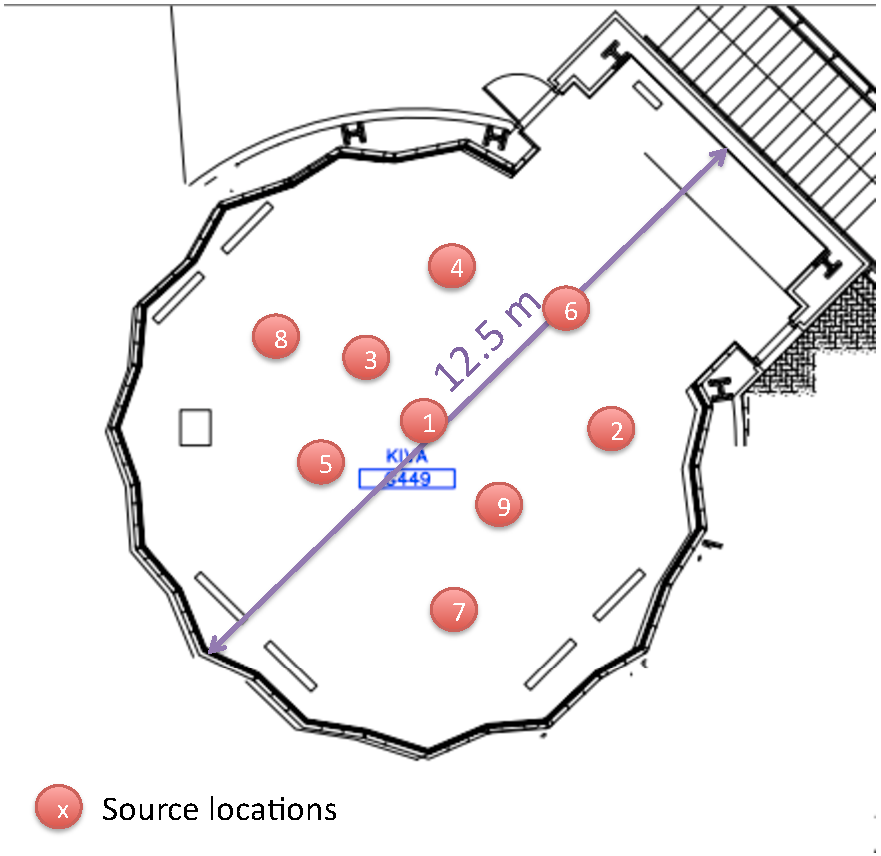
\includegraphics[width=4in]{img/testroom.pdf}}
\caption{Testroom floorplan and chemical vapor source locations.}
\label{fig:testroom}
\end{center}
\end{figure}

\begin{table}
\caption{Parameters of the experiment.}
\begin{center}
\begin{tabular}{|p{\tablewidthtwo}|p{\tablewidthtwo}|}
\hline
Chemical used as source & Liquid ethanol, 70\% \\ \hline
Surface area of chemical vapor source & 0.018 $\text{m}^2$\\ \hline
Vertical distance between sensor plane and
test room floor & 0.3 $\text{m}$ \\ \hline
Minimum initial distance between sensor and chemical & 2 $\text{m}$ \\ \hline
Radius of localization & 1.0 $\text{m}$ \\ \hline
Delay between robot start and source exposure & 30 minutes \\ \hline
Delay between source exposure and the start of a trial & 30 minutes \\ \hline
Duration of trial & 35 minutes \\ \hline
\end{tabular}
\end{center}
\label{tab:parameters}
\end{table}

\subsubsection{Test Procedure}
A single exposed dish of ethanol was placed in the test room at least 30
minutes before the start of each trial, and remained undisturbed at
its initial location for the entirety of the trial. The robot was
initialized at a random location no less than 2 meters away from the
location of the source, and operated  autonomously throughout
the trial.  The duration of each trial was 35 minutes, beginning when
the first chemical sensor reading was taken. 

Nine sets of two trials were conducted using the nine chemical source
locations shown in figure \ref{fig:testroom}.  For each source
location, one trial was conducted using the greedy planner, and one trial
was conducted using the stochastic planner.

When the location of the source was changed between trials, a waiting period of at least 2 hours
was allowed, during which no ethanol was exposed. According to regulations regarding the air
cycle rate for an office building, it was determined that the air in
the test room was replaced 4 times per hour.  Thus, it was assumed that a 2 hour waiting
period cleaned the room of ethanol traces.

\subsubsection{Data Acquisition}
All of the particles of the particle filter located less than a distance of 1 meter from the
true source location were considered to be within the ``localization
radius.''  The sum of the probabilities of the particles within the
localization radius at the beginning and end of each trial was used to
calculate the mean localization rate achieved in that trial by the
process described in section \ref{sec:results}.

The probabilities of all of the particles were logged each time the
posterior was updated, and the initial and final sums of probability
mass within the localization radius were calculated after the
end of each trial. Raw chemical sensor readings, robot position, planner commands, and
posterior estimates were also logged at a rate of 1 hz.

\newpage

\section{Results}
\label{sec:results}
The results of this experiment contradict the hypothesis presented in
section \ref{sec:hos}.  This section contains  a summary of experimental data
and detailed statistical analysis of the data to assess the
hypothesis.

\subsection{Experimental Data}
For each of the nine source locations, table \ref{tab:data} shows the
ratio of the localization rate of
a trial using the stochastic planner to the localization rate of
a trial using the simple gradient descent (greedy) planner, as well as
the raw quantities used to calculate this ratio. $m_0$ is the initial sum of
the probabilities of particle filter particles located inside the 1
meter localization radius for each trial, and $m_f$ is the final sum
of the probabilities of the same particles. The localization rate of
each trial is calculated according to the equation $rate =
\frac{m_f/m_0}{T_{trial}}$ where $T_{trial}$ is the length of the
trial in minutes.  The ratio $R$ is given by the equation $R =
\frac{rate_{stoch}}{rate_{greedy}}$ and serves as a numerical
comparison between the localization rate using the greedy planner and
the localization rate using the stochastic planner for each source location.

\begin{table}[htb]
\begin{center}
\begin{tabular}{|c||c||c||c||c||c||c||c||c||c|}
\hline
 Source Location & 1 & 2 & 3 & 4 & 5 & 6 & 7 & 8 & 9 \\
\hline \hline
$m_{0_{greedy}}$ & 0.0502 & 0.0450 & 0.0500 & 0.0500 & 0.0497 & 0.0481 & 0.0493 & 0.0506 & 0.0497 \\
\hline
$m_{f_{greedy}}$ & 0.0468 & 0.0451 & 0.2935 & 0.0511 & 0.0519 & 0.0492 & 0.0562 & 0.0503 & 0.0518 \\
\hline
$r_{greedy}$ & 0.0259 & 0.0286 & 0.1656 & 0.0282 & 0.0298 & 0.0286 & 0.0303 & 0.0280 & 0.0293 \\
\hline
$m_{0_{stoch}}$ & 0.0502 & 0.0450 & 0.0500 & 0.0500 & 0.0497 & 0.0484 & 0.0493 & 0.0506 & 0.0490 \\
\hline
$m_{f_{stoch}}$ & 0.0521 & 0.0483 & 0.0525 & 0.0491 & 0.0480 & 0.0488 & 0.0495 & 0.0515 & 0.0491 \\
\hline
$r_{stoch}$ & 0.0295 & 0.0296 & 0.0299 & 0.0279 & 0.0268 & 0.0272 & 0.0280 & 0.0285 & 0.0280 \\
\hline
\hline
$R = \frac{rate_{stoch}}{rate_{greedy}}$  & 1.1371 & 1.0345 & 0.1807 & 0.9869 &
0.9014 & 0.9505  & 0.9251 & 1.0164 & 0.9564\\
\hline
\end{tabular}
\caption{Experimental Data \label{tab:data} }
\end{center}
\end{table}

The mean $R_{mean}$ of the ratios $R$ for the nine source locations is equal to
$R_{mean} = 0.8989$ and was used to assess the hypotheis as false. The
90\% confidence interval on $R_{mean}$ is $(0.7263, 1.0714)$.

\subsection{Statistical Hypothesis Assessment}
A one-sided Student's t-test with 8 degrees of freedom on alternative
hypothesis $R_{mean} > 1.2$ gave a t-statistic of $-3.2466$ with a
corresponding p-value of $0.9941$.  Thus, the probabilty of
obtaining a measured ratio greater than or equal to $R_{mean} = 0.8989$
is $99.4\%$ under the null hypothesis ($R_{mean} = 1.2$), so the
alternative hypothesis $R_{mean} > 1.2$ must be rejected.  Figure
\ref{fig:killer} shows a graphical representation of the experimental
data and the rejected hypothesis.

\begin{figure}
\begin{center}
\fbox{
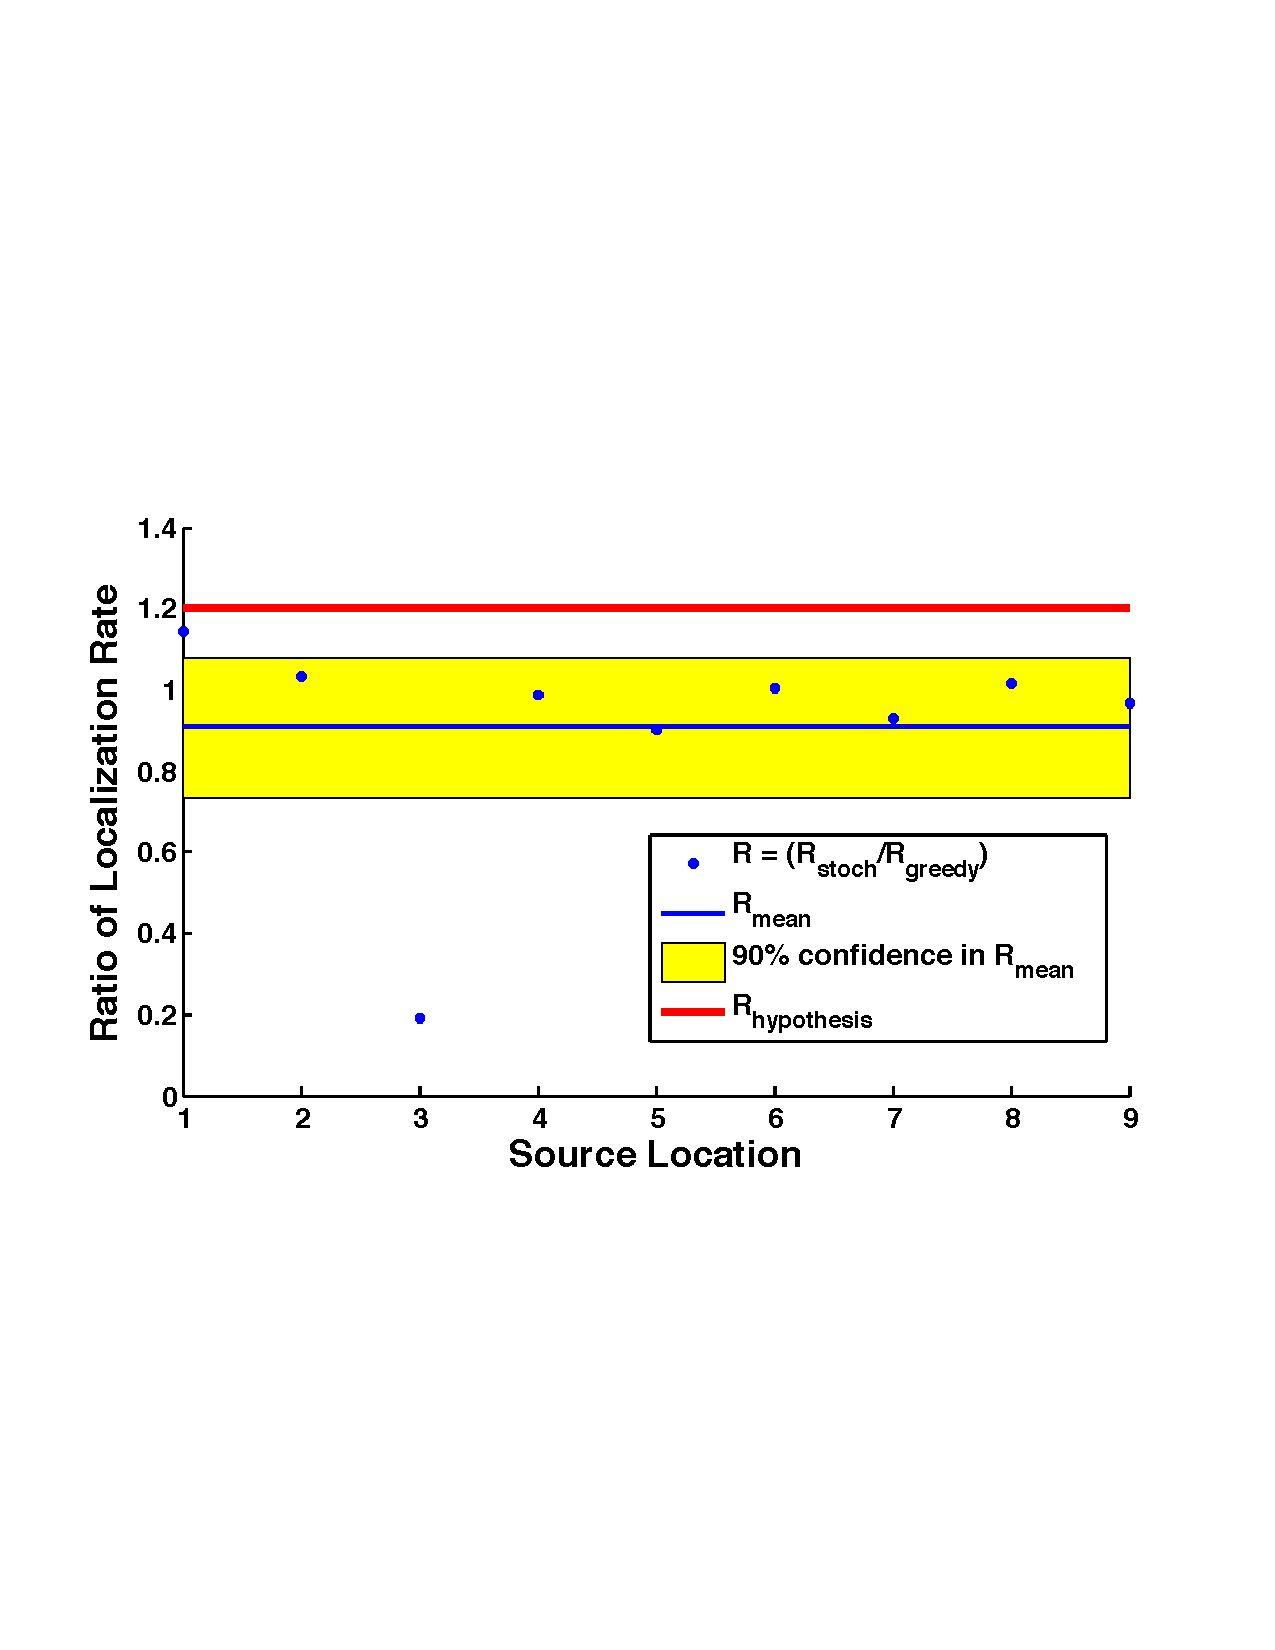
\includegraphics[width=6in]{img/Killer.pdf}}
\caption{Graphical representation of data and hypothesis.}
\label{fig:killer}
\end{center}
\end{figure}


\subsection{Additional Assessment of Results}
\label{sec:additional}
In addition to the assessment of the hypothesis, a two-sided Student's
t-test with 8 degrees of freedom was used on the hypothesis $R_{mean}
= 1$ to determine whether there was any statistically significant
difference in the mean localization rates.  This test gave
a t-statistic of $-1.0903$ and a p-value of $0.3073$, showing that
there is no statistically significant difference in the mean localization
rate achieved with the stochastic planner and the rate achieved with
the simple gradient descent planner.

\section{Discussion}
As described in the previous section, the stochastic planner was not
shown to produce a higher mean localization
rate than the simple gradient descent planner.  One possible cause may
have been
that the system did not produce a statistically significant increase
in the sum of probability mass inside the localization radius using
either planner.  The results of a two-sided Student's t-test on the
null hypothesis $\frac{m_f}{m_0} = 1$ are given in table
\ref{tab:nofind}.  Although the t-statistics show some increase in the
sum of probability mass inside the localization radius,
particularly in the case of the stochastic planner, this increase is
not significant at a 10\% level.

\begin{table}[htb]
\begin{center}
\begin{tabular}{|c||c|c|}
\hline
& t-statistic & p-value \\
\hline \hline
Greedy Planner & 1.0296 & 0.3333\\
\hline
Stochastic Planner& 1.3994 &0.1993\\
\hline
\end{tabular}
\caption[Student's t-test on probability mass increase inside
localization radius.]{Student's t-test for an increase in the sum of probability
  mass inside the localization radius over the time of a trial.
  These results show no statistically significant increase. \label{tab:nofind} }
\end{center}
\end{table}


One reason that the probability mass inside the localization
radius was not shown to increase over the time of a trial may have been
the presence of air currents in the room due to the ventilation
system, the motion of the robot, and other random disturbances. Currents may have invalidated the
assumption that the air directly above the true source location
holds a higher chemical vapor concentration than all surrounding
points.  A qualitative drifting behavior was observed in carrying out
the experiment, where higher concentration measurements were taken
at a distance of one to two meters in one direction from the source than were
taken at similar distances in other directions, and even at the exact
source location.  Further experimental characterization of indoor
chemical dispersion is necessary to confirm this drifting
behavior quantitatively.  The robotic localization system tested in
this experiment attempts to localize the area of highest
concentration, since the estimation algorithms assume the area of highest
concentration to be the location of the true source.  If the true
source location is in fact different from the location of the
highest chemical vapor concentration, the system may not be able to accurately
localize the source, regardless of which planner is used.  The
possibility of system failure in the manner described represents a lack of robust estimation techniques, and
calls for further research in the area of estimation algorithms for
indoor robotic odor localization.

The stochastic planner was expected to produce a greater localization
rate than the simple gradient descent planner due to the fact that it
was expected to gather concentration measurements from a larger
percentage of the test room area.  In experimental trials with the
stochastic planner, the system did gather measurements from a larger
area than in trials with the greedy planner.  This result is shown
qualitatively by the comparison of robot paths in figure \ref{fig:paths} and
quantitatively in table \ref{tab:paths}, where $A_{greedy}$ and
$A_{stoch}$ are the percentage of the area of the test room ``covered''
using the greedy planner and the stochastic planner respectively.  For
the purpose of this analysis, the covered area is calculated by area the convex hull
of the set of locations that the robot took measurements at, i.e., the area of
the smallest convex shape that includes all the measurement locations.

\begin{figure}
\begin{center}
\fbox{
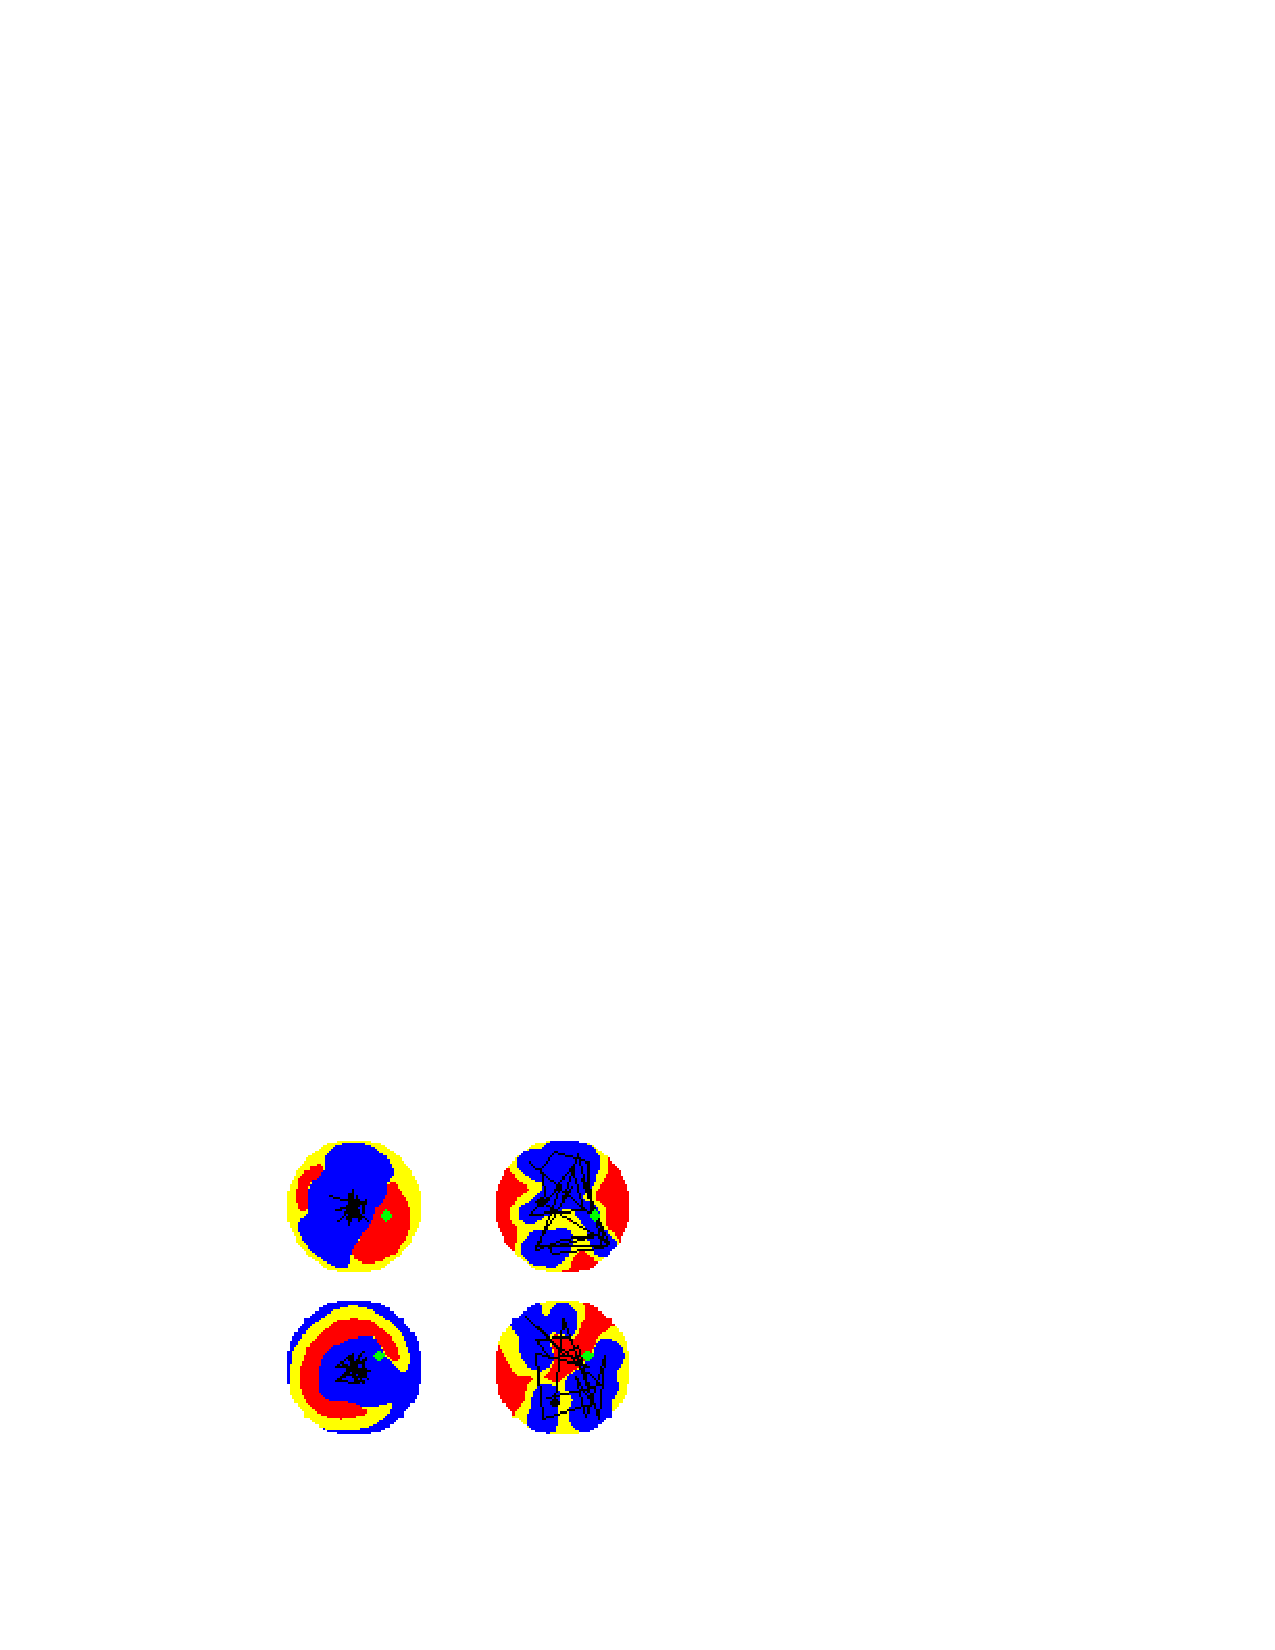
\includegraphics[width=6in]{img/paths.pdf}}
\caption[Final posterior estimates for source locations 7 and 8]{Comparison of robot paths and resulting final particle filter
  probability distributions using the greedy planner (left) and the
  stochastic planner (right) for source locations 7 (top) and 8 (bottom). The
  robot paths are shown in black, where each corner represents a
  measurement location, and the true source locations are
  shown in green.  The circular color fields represent the particle
  filter probability distributions.  The particles making up the top 25\% of the
  probability mass is shown in red, the particles making up the next
  25\% are shown in yellow, and the bottom 50\% are shown in blue. It
  is clear that the different planners produce different distributions
of measurements over the space in the test room, and this results in
different final particle filter probability distributions.}
\label{fig:paths}
\end{center}
\end{figure}

\begin{table}[htb]
\begin{center}
\begin{tabular}{|c||c||c||c||c||c||c||c||c||c|}
\hline
 Source Location & 1 & 2 & 3 & 4 & 5 & 6 & 7 & 8 & 9 \\
\hline \hline
$A_{greedy}$ & 0.1006 & 0.0750 & 0.237 & 0.0775 & 0.0802 & 0.1042 & 0.0669 & 0.0561 & 0.0612 \\
\hline
$A_{stoch}$ & 0.4940 & 0.4523 & 0.5405 & 0.5278 & 0.5032 & 0.5717 & 0.4930 & 0.5469 & 0.5311 \\
\hline
\end{tabular}
\caption{Percentage of possible area covered by the different planning algorithms.}
\label{tab:paths}
\end{center}
\end{table}

The differences in the distribution of measurement locations over the test room
produced by the greedy planner and the stochastic planner caused the
two planners
to produce different final particle filter probability distributions,
as illustrated qualitatively in figure \ref{tab:paths}.  However, as
discussed in section \ref{sec:results}, the difference in final
probability distributions did not produce a statistically significant
difference in the localization rate.  As discussed earlier in this
section, it is possible that the point of highest concentration is
not the true source location.  If this is the case, the use of a localization radius about
the true source location
to determine the localization rate may not fully assess the
relative performance of the two planners.  Though the use of a
localization radius accurately
assesses the performance of the system in localizing the true source,
and thus correctly and accurately assesses the hypothesis, this metric only takes
into account a subset of the information gained by the particle filter
during a trial.

It is feasible that a more robust estimation technique could be developed through
future research that takes into account any differences that may exist
between the true source location and the location of highest chemical
vapor concentration.  To gain preliminary intuition regarding the
relative performance of the simple gradient descent planner and the
stochastic planner in such a circumstance, it was desired to know
whether there was any difference between the full amount of information
gained in a trial using the greedy planner, and the amount gained
using a stochastic planner.  The amount of information gained in each
trial was measured by calculating the Kullback – Leibler divergence (KL
divergence) of
the final particle filter probability distribution from the initial
uniform distribution where all of the particles are assigned the same
probability.  The KL divergence of the particle filter probability
distribution in each trial is shown in table \ref{tab:allinfo}.

\begin{table}[htb]
\begin{center}
\begin{tabular}{|c||c||c||c||c||c||c||c||c||c|}
\hline
 Source Location & 1 & 2 & 3 & 4 & 5 & 6 & 7 & 8 & 9 \\
\hline \hline
$KL_{greedy}$  & 0.0029 & 0.0019 & 0.3156 & 0.0024 & 0.0071 & 0.0007 & 0.0070 & 0.0039 & 0.0085 \\
\hline
$KL_{stochastic}$ & 0.0013 & 0.0082 & 0.0017 & 0.0015 & 0.0030 & 0.0019 & 0.0012 & 0.0008 & 0.0011 \\
\hline
$\frac{KL_{stoch}}{KL_{greedy}}$ & 0.4463 & 4.3945 & 0.0052 & 0.6107 & 0.4157 & 2.7365 & 0.1711 & 0.1990 & 0.1282 \\
\hline
\end{tabular}
\caption[KL divergence of posterior distribution from a uniform distribution]{Kullback-Leibler divergence of the final particle filter
  probability distribution from the initial uniform particle
  probability distribution.  This is a measure of how much
  information about the environment was gained by the system in each trial. }
\label{tab:allinfo}
\end{center}
\end{table}

The mean of the ratios $\frac{KL_{stoch}}{KL_{greedy}}$ over the 9
source locations is equal to $mean(\frac{KL_{stoch}}{KL_{greedy}}) =
1.0119$.  A two-sided Student's t-test with the null hypothesis
$mean(\frac{KL_{stoch}}{KL_{greedy}}) = 1$ gave a t-statistic of
$0.0235$ and a p-value of $0.9818$.  This shows there is no significant
difference in the information gain between the two.

The important metric is not general information gain, however, but is the gain
of information about the source location. There are other metrics that use the
information from all of the particles to measure how well the source location
has been estimated. 

Table \ref{tab:weighted-distance} shows the probabilistic weighted distances
of the true source location to the posterior estimate.  The weighted distance is
calculated by taking the weighted average distance from each particle location
to the source location, where the weighting for each particle is determined by the
probability mass held by the particle at the end of a trial.  A two-sided
Student's t-test on the ratio of the stochastic to the greedy weighted distance
shows that the ratio is not statistically significantly different from 1,
resulting in a t-statistic of $0.8862$ and a p-value of $0.4014$. If, however,
we look at all the source locations where one of the planners did not
definitively find the source, i.e. all the source locations other than source
location 3, the ratio of the weighted distances is significantly different from
1. Running the same Student's t-test over the other 8 source location gives a
t-statistic of $-2.4529$ and a p-value of $0.0439$. This is statistically
significant difference from 1 at the $5\%$ level. This difference is not
overwhelming, as the mean ratio of the weighted distances is $0.9948$, but at a
minimum this shows that by covering more of the search space the stochastic planner
lowers the probability of more areas being potential source locations.

% \begin{table}[htb]
% \begin{center}
% \begin{tabular}{|c||c||c||c||c||c||c||c||c||c|}
% \hline
%  Source Location & 1 & 2 & 3 & 4 & 5 & 6 & 7 & 8 & 9 \\
% \hline \hline
% Greedy KL divergence & 1.3819 & 1.8294 & 0.6025 & 1.4937 & 1.4636 & 1.3319 & 1.3668 & 1.3803 & 1.5682 \\
% \hline
% Stochastic KL divergence & 1.2861 & 1.7989 & 1.2882 & 1.5312 & 1.5107 & 1.3297 & 1.3736 & 1.3431 & 1.5974 \\
% \hline
% Ratio $\frac{KL_{stoch}}{KL_{greedy}}$ & 0.9306 & 0.9833 & 2.1381 & 1.0251 & 1.0322 & 0.9984 & 1.0050 & 0.9730 & 1.0186 \\
% \hline
% \end{tabular}
% \caption{Kullback-Leibler divergence of the final particle filter
%   posterior distribution from an 'ideal' Gaussion posterior distribution . }
% \label{tab:kl-ideal}
% \end{center}
% \end{table}


\begin{table}[htb]
\begin{center}
\begin{tabular}{|c||c||c||c||c||c||c||c||c||c|}
\hline
 Source Location & 1 & 2 & 3 & 4 & 5 & 6 & 7 & 8 & 9 \\
\hline \hline
$D_{greedy}$ & 3.0630 & 4.5139 & 2.1940 & 3.9041 & 3.8425 & 3.2819 & 3.5805 & 3.4443 & 4.0892 \\
\hline
$D_{stoch}$ & 3.0180 & 4.4869 & 3.0832 & 3.9119 & 3.8311 & 3.2875 & 3.5517 & 3.4059 & 4.0805 \\
\hline
$\frac{D_{stoch}}{D_{greedy}}$ & 0.9853 & 0.9940 & 1.4053 & 1.0020 & 0.9971 & 1.0017 & 0.9920 & 0.9888 & 0.9979 \\
\hline
\end{tabular}
\caption[Probabilistically weighted distance from the posterior estimate to the
source location]{Weighted distance of the posterior particle distribution from the true
  source location. The weighted distance is the average of the distances from
  each particle location to the source location weighted by the probability
  mass of the posterior held by that particle.}
\label{tab:weighted-distance}
\end{center}
\end{table}

\section{Summary and Conclusion}

\section{Acknowledgments}

\newpage
\bibliographystyle{aiaa}
\bibliography{sources}
\nocite{*}

\end{document}